	\begin{figure}[H]
		\newcommand{\robot}[4]{
			\begin{scope}[shift={(#1,#2)}, scale=#3]

				% Head
				\draw[rounded corners=3pt, fill=gray!20] (-1,1)
				rectangle (1,3);

				% Eyes (use color parameter)
				\fill[#4] (-0.5,2.2) circle (0.15);
				\fill[#4] (0.5,2.2) circle (0.15);

				% Mouth
				\draw[line width=0.8pt] (-0.4,1.6) -- (0.4,1.6);

				% Antenna
				\draw[line width=0.8pt] (0,3) -- (0,3.6);
				\fill[#4] (0,3.6) circle (0.15);

				% Body
				\draw[rounded corners=5pt, fill=gray!10]
				(-1.5,-1) rectangle (1.5,1);

				% Buttons (also colored)
				\fill[#4] (0,0.3) circle (0.15);
				\fill[#4] (0,-0.2) circle (0.15);
				\fill[#4] (0,-0.7) circle (0.15);

				% Arms
				\draw[line width=0.8pt] (-1.5,0.5) -- (-2.2,0.5);
				\draw[line width=0.8pt] (1.5,0.5) -- (2.2,0.5);

				% Hands
				\fill[#4] (-2.2,0.5) circle (0.12);
				\fill[#4] (2.2,0.5) circle (0.12);

				% Legs
				\draw[line width=0.8pt] (-0.6,-1) -- (-0.6,-2);
				\draw[line width=0.8pt] (0.6,-1) -- (0.6,-2);

				% Feet
				\draw[line width=1.5pt] (-0.9,-2) -- (-0.3,-2);
				\draw[line width=1.5pt] (0.3,-2) -- (0.9,-2);

			\end{scope}
		}
		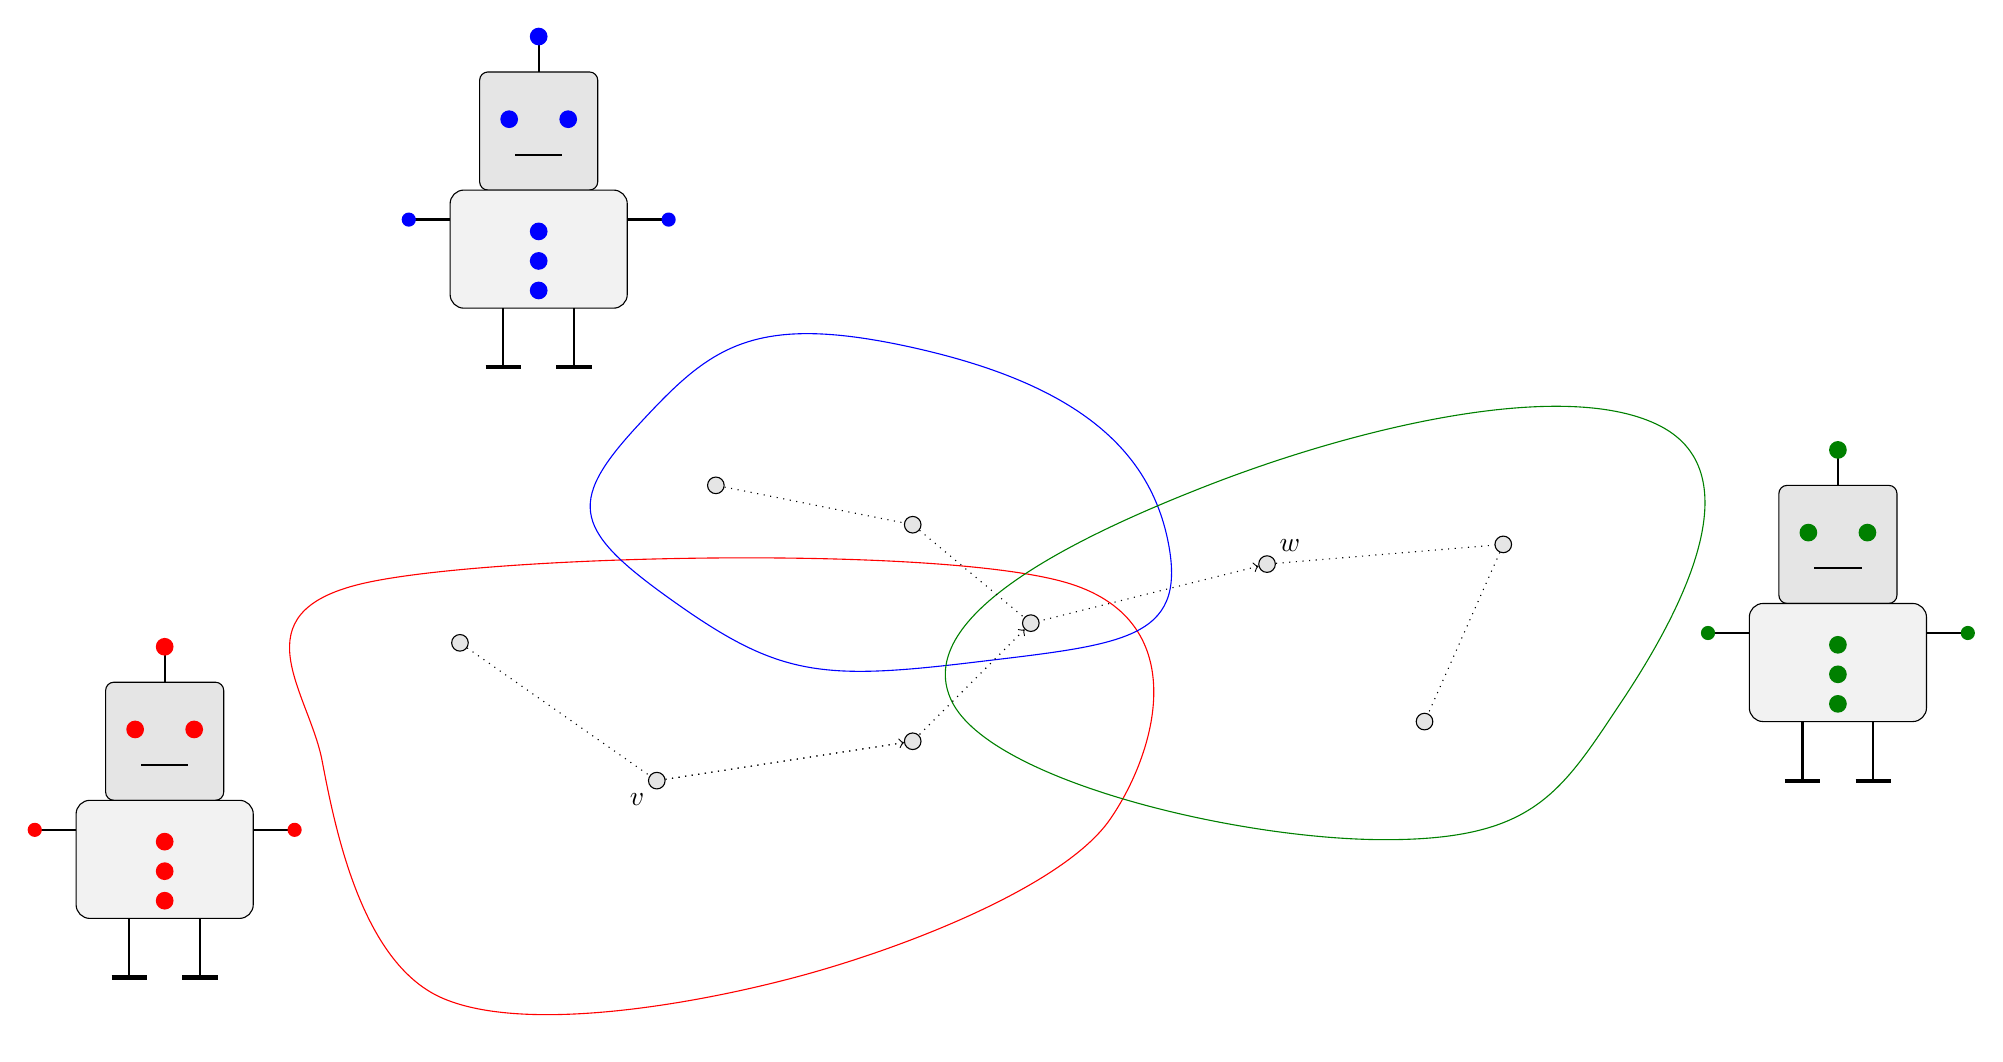
\begin{tikzpicture}[
			scale=2.5,  
			vertex/.style={
				circle,
				draw,
				fill=black!10,
				minimum size=6pt,
				inner sep=0pt
			}
			]

			% Subgraph boundaries

			\robot{-3}{-1}{0.3}{red}
			\draw[red] plot [smooth cycle, tension=0.6] coordinates
			{(-2.2,-0.5) (-2,0.4) (1.6,0.4)  (1.8,-0.8) (0.2,-1.6) (-1.6,-1.7)};

			\robot{-1.1}{2.1}{0.3}{blue}
			\draw[blue]  plot [smooth cycle, tension=1.1] coordinates
			{(-0.6,1.2) (0.8,1.6) (2.1,0.6) (1.1,0) (-0.4,0.3)};

			\robot{5.5}{0}{0.3}{green!50!black}
			\draw[green!50!black] plot [smooth cycle, tension=0.8] coordinates
			{(2.3,0.9) (4.6,1.2) (4.4,-0.2) (3.2,-0.9) (1.0,-0.2)};

			% G1 vertices
			\node[vertex] (a1) at (-1.5,0.1) {};
			\node[vertex] (a2) at (-0.5,-0.6) {};
			\node[vertex] (a3) at (0.8,-0.4) {};
			\draw[dotted] (a1) -- (a2) -- (a3);

			% G2 vertices
			\node[vertex] (b1) at (-0.2,0.9) {};
			\node[vertex] (b2) at (0.8,0.7) {};
			\node[vertex] (b3) at (1.4,0.2) {};
			\draw[dotted] (b1) -- (b2) -- (b3);

			% G3 vertices
			\node[vertex] (c1) at (2.6,0.5) {};
			\node[vertex] (c2) at (3.8,0.6) {};
			\node[vertex] (c3) at (3.4,-0.3) {};
			\draw[dotted] (c1) -- (c2) -- (c3);

			% Labels
			\node[below left=1pt] at (a2) {$v$};
			\node[above right=1pt] at (c1) {$w$};

			% Cross connections
			\draw[dotted, <-] (c1) -- (b3);
			\draw[dotted, <-] (b3) -- (a3);
			\draw[dotted, <-] (a3) -- (a2);


		\end{tikzpicture}
		\caption{Multiple learning agents with graph ownership}
	\end{figure}
